\chapter{Methods}
\label{chap:methods}

In this chapter, the methods used in this thesis are described.

\section{Optical Character Recognition}
\label{sec:ocr}

In this section, the \gls{ocr} methods used in this thesis are described.

\subsection{EasyOCR}
\label{subsec:easyocr}

EasyOCR is a Python library for \gls{ocr} \cite{easyocr_2020}. It uses a deep learning model to detect text.

\subsection{Tesseract}
\label{subsec:tesseract}

Tesseract is an \gls{ocr} engine \cite{tesseract_2007}. It is open-source and was developed by Google. It is written in C++ and has a Python wrapper.

\subsection{Other Optical Character Recognition Methods}
\label{subsec:other_ocr_methods}

We don't use other \gls{ocr} methods in this thesis.
However, we mention them here for completeness.


\section{Metrics}
\label{sec:metrics}

In this section, we go over the metrics used in this thesis.

\subsection{Character Error Rate}
\label{subsec:cer}

The \gls{cer} describes how many substitutions, deletions, and insertions are necessary to transform a text prediction into the text label.
It is defined as follows:

\begin{equation}
    \text{CER} = \frac{S + D + I}{N}
    \label{eq:cer}
\end{equation}
with \(S\) being the number of substitutions, \(D\) the number of deletions, \(I\) the number of insertions, and \(N\) the total number of characters of the label.
The \gls{cer} ranges from 0 to $\infty$, where 0 means perfect recognition and the higher the worse the recognition.
Because the \gls{mos} is defined in the range 0 to 100 and 100 represents a high subjective quality, the two metrics are unintuitive to compare.
Therefore, we are transforming the CER by subtracting it from 1 and multiplying it by 100 to get a \gls{mos}-like value, see \autoref{eq:cer2mos}.

\begin{equation}
    \text{CER}_{comp} = (1 - \text{CER}) \cdot 100.
    \label{eq:cer2mos}
\end{equation}

This means that the $\text{CER}_{comp}$ can be in the range -$\infty$ to 100, where 100 means perfect recognition and the lower the worse the recognition.
Although the $\text{CER}_{comp}$ is generally in the range 0 to 100, which matches the \gls{mos}.

\subsection{Peak Signal-to-Noise Ratio}
\label{subsec:psnr}

The \gls{psnr} \cite{PSNRvsSSIM_2010} describes the ratio of the maximum possible power of a signal and the power of corrupting noise that affects it.
When it is applied to an image, the \gls{psnr} is defined as follows:

\begin{equation}
    \text{PSNR} = 10 \cdot \log_{10} \left( \frac{R^2}{\text{MSE}} \right)
    \label{eq:psnr}
\end{equation}

with \(R\) being the maximum possible pixel value of the image and \gls{mse} being the mean squared error between the original and the reconstructed image.

\subsection{Bjøntegaard Delta Rate}
\label{subsec:bdrate}

The \gls{bdrate} \cite{bdrate_original_2001}\cite{bdrate_beyond_2022} (can't find pdf of original paper) is defined by the difference between the integration of curves of the codecs to compare.
The first curve is the reference curve and the second the test curve.
Both are plotting some average metric over the average bitrate of some images.

\begin{equation}
    \text{BDRate} = https://arxiv.org/pdf/2202.12565.pdf
    \label{eq:bdrate}
\end{equation}

\section{Codecs}
\label{sec:codecs}

In this section, the codecs used in this thesis are described.

\subsection{High Efficiency Video Coding}
\label{subsec:hevc}

\gls{hevc} is a video codec.

\subsection{Versatile Video Coding}
\label{subsec:vvc}

\gls{vvc} is a video codec.


\section{Correlation}
\label{sec:correlation}

In this section, we describe the correlation methods we use to compare the behavior of the \gls{mos} and the \gls{cer}.
These can then be used to determine if the \gls{cer} is a good alternative for the \gls{mos}.

\subsection{Pearson Correlation}
\label{subsec:pearson}

The \gls{plcc} \cite{pears_spear_2016} describes the linear correlation between two variables, normalized to the range \([-1, 1]\).
It is defined as follows:

\begin{equation}
    r_p = \frac{\sum{(x-m_x)(y-m_y)}}{\sqrt{\sum{(x-m_x)^2}\sum{(y-m_y)^2}}}
    \label{eq:pearson}
\end{equation}

with \(x\) and \(y\) being the two vectors, \(m_x\) and \(m_y\) being the mean of \(x\) and \(y\), respectively.
If the \gls{plcc} is close to 1, the two vectors have a positive linear relationship, which means that if \(x\) increases, \(y\) increases as well.
If the \gls{plcc} is close to -1, the two vectors have a negative linear relationship, which means that if \(x\) increases, \(y\) decreases.
If the \gls{plcc} is close to 0, the two vectors have no correlation at all.

\subsection{Spearman Ranked Correlation}
\label{subsec:spearman}

The \gls{srcc} \cite{pears_spear_2016} describes the monotonic correlation between two variables, normalized to the range \([-1, 1]\).
Compared to the \gls{plcc}, it mainly takes the order/rank of the values into account, not the exact values.
The Spearman ranked correlation is defined as follows:

\begin{equation}
    r_s = \frac{\sum{(R_X-m_{R_X})(R_Y-m_{R_Y})}}{\sqrt{\sum{(R_X-m_{R_X})^2}\sum{(R_Y-m_{R_Y})^2}}}
    \label{eq:spearman}
\end{equation}

with \(R_X\) and \(R_Y\) being the two vectors of the ranks of \(x\) and \(y\), respectively, and \(m_{R_X}\) and \(m_{R_Y}\) being the mean of \(R_X\) and \(R_Y\), respectively.
If the \gls{srcc} is close to 1, the two vectors have a positive monotonic relationship, which means that the rank of \(x\) increases, the rank of \(y\) increases as well.
If the \gls{srcc} is close to -1, the two vectors have a negative monotonic relationship, which means that the rank of \(x\) increases, the rank of \(y\) decreases.
If the \gls{srcc} is close to 0, the ranks of the two vectors have no correlation at all.
These characteristics will help us, to determine if the \gls{cer} is a good alternative for the \gls{mos}, by checking how similar the ranks of the two metrics are.

\section{Nonlinear Transformation}
\label{sec:nonlinear}

In this section, we describe the nonlinear curve fitting used to transform the \gls{mos} to better fit the \gls{cer}.
This is mainly done because the subjective scores have been found to be not reliable \cite{nonlin_fit_original_2000}.
The model we used was defined in \cite{nonlin_fit_original_2000}.
The Authors suggest an extension to the model, which we leave out for simplicity.
It is defined as follows:

\begin{equation}
    \text{MOS}_{trans} = \frac{a - b}{1 + \exp \left( \frac{-\text{MOS} + c}{d} \right)} + b
    \label{eq:nonlinear}
\end{equation}
    
The parameters are initialized as follows:
\begin{equation}
    \begin{aligned}
        a &= \max{CER} \\
        b &= \min{CER} \\
        c &= \overline{MOS} \\
        d &= 1
    \end{aligned}
    \label{eq:nonlinear_init}
\end{equation}
We fit the parameters \(a\), \(b\), \(c\), and \(d\) to the data of all the images with the help of the least squares method.
We then use the model and the \gls{cer} values the predict the transformed \gls{mos} values.
A similar transformation was used in \cite{nonlin_fit_2011}\cite{nonlin_fit_appl_2017}.

\begin{figure}[h]
    \centering
    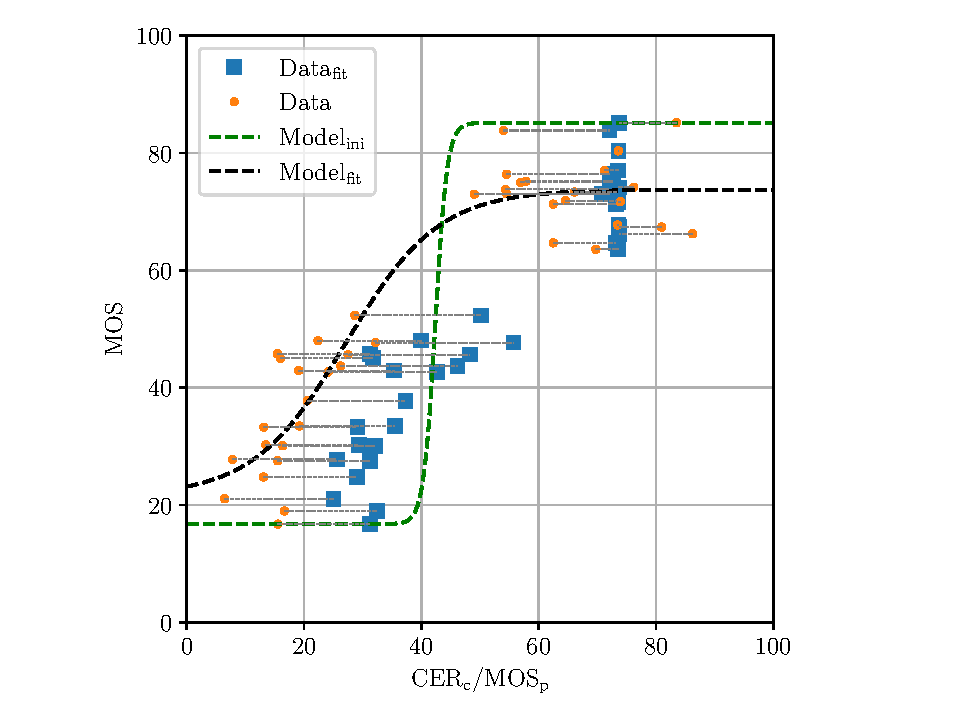
\includegraphics[width=\textwidth]{../exp/fit_example.pdf}
    \caption{Example of the nonlinear fit with subjective and objective values}
    \label{fig:nonlinear_fit}
\end{figure}

In Figure \ref{fig:nonlinear_fit}, we can see an example of the nonlinear fit.
First we have some random data from subjective and objective values, which might represent the \gls{mos} and \gls{cer} values of some images.
We then use the model and the parameters and fit the model to the data.
The fitted curve clearly fits the data better than the curve with the initial parameters.
Additionally we can calculate the \gls{plcc} and \gls{srcc} of the two curves.
We see that the \gls{plcc} and \gls{srcc} of the fitted curve are higher than the \gls{plcc} and \gls{srcc} of the curve with the initial parameters.
With the \gls{plcc} it is not as obvious to see, but for the \gls{srcc} we can clearly see that the fitted curve is monotonic, while some of the initial datapoints are ranked first on the subjective value, but a higher rank on the objective value.
This leads to a \gls{srcc} of 1 for the fitted data, but a slightly lower \gls{srcc} for the initial data.

We can use this method later to transform the \gls{mos} to improve the correlation with the \gls{cer}.
